\documentclass{CV_template}

%===============================================================================================%
%   CONTENIDO DEL DOCUMENTO
%===============================================================================================%

\begin{document}

\columnratio{0.3} % Donde comienza la siguiente columna de texto.
\setlength{\columnsep}{2em} % Sangria de la siguiente columna de texto.
\setlength{\columnseprule}{4pt} % Linea vertical entre columnas y su espesor.
\colseprulecolor{maingray} % Color de la linea vertical.

\begin{paracol}{2}

%===============================================================================================%
%   BARRA LATERAL
%===============================================================================================%

\begin{leftcolumn}

    \begin{figure}[t]
        \centering
        \noindent    
        \begin{tikzpicture}[remember picture,overlay]
            \node [rectangle, fill=sidecolor, anchor=north, minimum width=16.5cm, minimum height=\paperheight+1cm] (box) at (-5cm,0.5cm){};
        \end{tikzpicture}    
        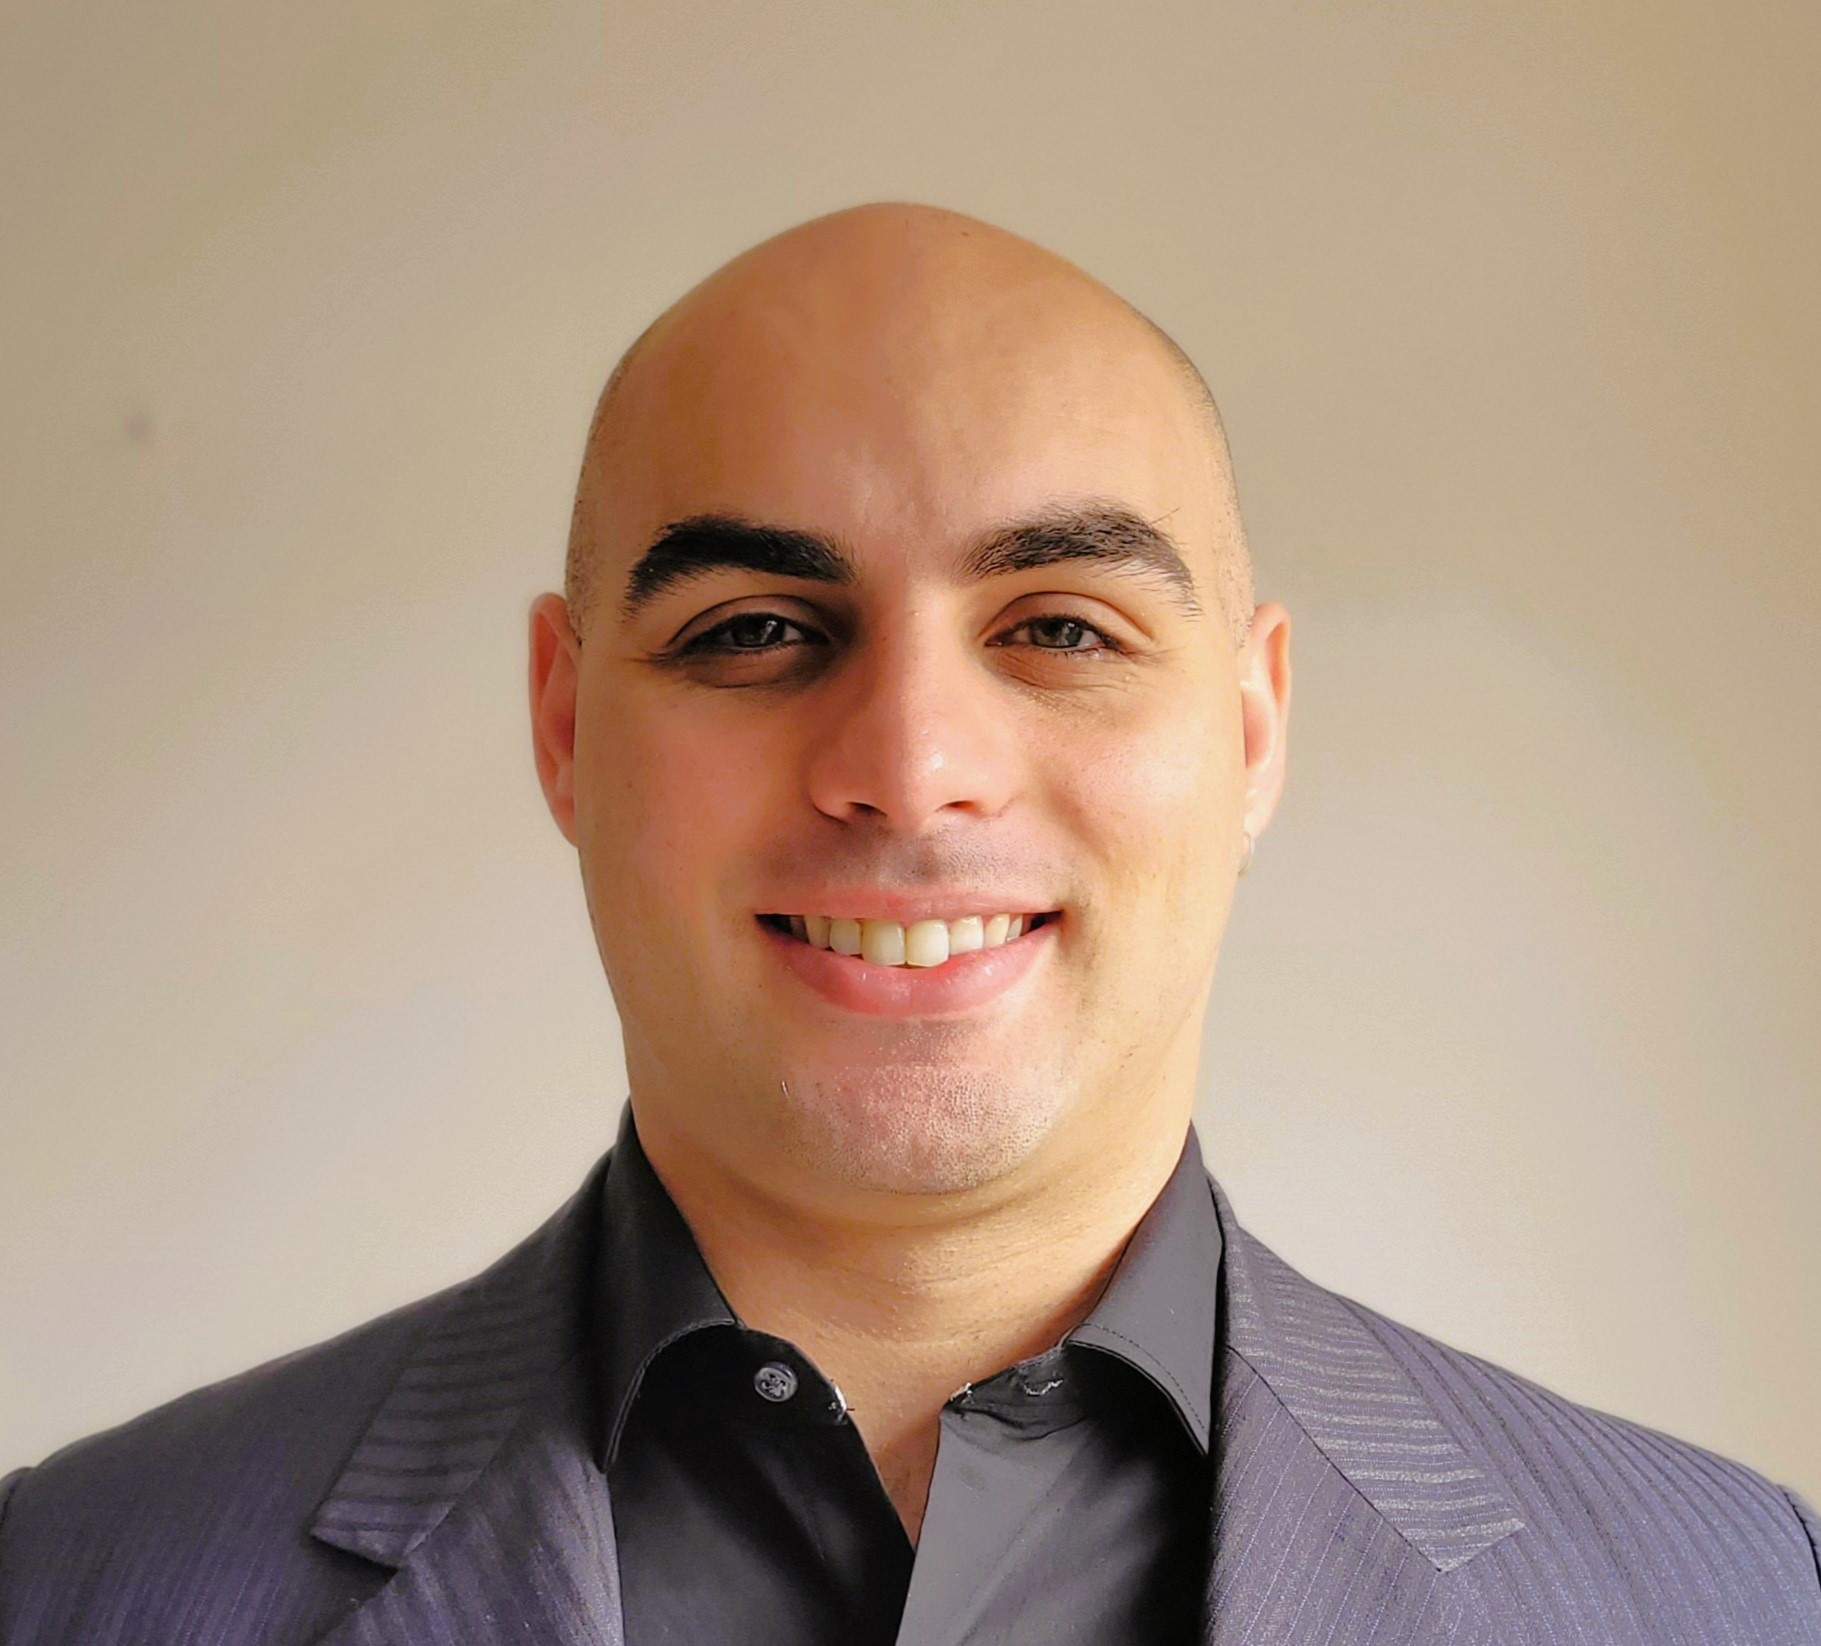
\includegraphics[width=\linewidth]{Foto.jpg}
    \end{figure}
    
    \cvsection{CONTACTO}

    \begin{tabular}{cl}
        {\Large\color{maincol}\faCalendar}                        & 01 de abril de 1992                                                       \\ [2pt]
        \multirow{2}{*}{{\Large\color{maincol}\faInfoCircle}}     & \href{https://goo.gl/maps/ciK9KomkCkJ7PdWt5}{Bahía Blanca Buenos Aires,} \\ [2pt]
                                                                  & \href{https://goo.gl/maps/ciK9KomkCkJ7PdWt5}{Argentina {\footnotesize\faExternalLink}}                   \\ [2pt]
        {\Large\color{maincol}\faAt}                              & \href{mailto:juanmcarini@gmail.com}{juanmcarini@gmail.com}                \\ [2pt]
        {\Large\color{maincol}\faPhone}                           & +54 (0291) 414 3811                            \\ [2pt]
        {\Large\color{maincol}\faGithub}                          & \href{https://github.com/JuanMCarini}{JuanMCarini {\footnotesize\faExternalLink}}                        \\ [2pt]
        {\Large\color{maincol}\faLinkedinSquare}                  & \href{https://www.linkedin.com/in/juanmcarini}{juanmcarini {\footnotesize\faExternalLink}}
    \end{tabular}

    \cvsection{IDIOMAS}

    \begin{tabular}{ll}
        \textbf{Español:} & nativo \\ [2pt]
        \textbf{Ingles:}  & básico profesional.
    \end{tabular}

    \cvsection{HABILIDADES}

    \cvskill{SQL}      {0.3} 
    \cvskill{Python}   {0.4}
    \cvskill{Power BI} {0.5}
    \cvskill{Excel}    {0.8}
    \cvskill{\LaTeX}    {0.8}

\end{leftcolumn}

\begin{rightcolumn}
%===============================================================================================%
%   CABECERA
%===============================================================================================%
\fcolorbox{white}{darkcol}{\begin{minipage}[c][3cm][c]{0.99\mpwidth}
	\begin{center}
		\HUGE{ \textbf{ \textcolor{white}{ \uppercase{JUAN MARTÍN CARINI} } } } \\[-50pt]
		\textcolor{white}{ \rule{0.1\textwidth}{1.25pt} } \\[4pt]
		\large{\textcolor{white} {Lic.\@ en Matemática \& Científico de Datos}}
	\end{center}
\end{minipage}}
\vspace{6pt}

\cvsection{EDUCACIÓN}

    \itemedu{Data Science}
    {Marzo 2022 a la actualidad}{Coderhouse}
    \itemedu{\href{https://1drv.ms/b/s!Anr_tvZIYrhwgel_E2d7lqyOWQMaaQ}
            {Licenciatura en Matemática \normalfont{\footnotesize\faExternalLink}}}
            {Marzo 2010 a agosto de 2022}{Universidad Nacional del Sur}        
    \vspace{-6pt}
    \hspace{0.2cm}\textit{\small\textbf{Materias Optativas:}}
        \begin{itemize}
            \footnotesize
            \item \href{https://1drv.ms/b/s!Anr_tvZIYrhwg-Q3BLmxwlzX5PWIFQ}{Principios de Computación I  {\footnotesize\faExternalLink}},
            \item \href{https://1drv.ms/b/s!Anr_tvZIYrhwg-Q45aG0UgNb-R70FA?e=44lo7C}{Introducción a los procesos estocásticos  {\footnotesize\faExternalLink}}.
        \end{itemize} 

    \itemedu{\href{https://www.coderhouse.com/certificados/620447e524e5820051a7aa74}
            {Data Analytics \normalfont{\footnotesize\faExternalLink}}}
            {Noviembre 2021 a febrero de 2022}{Coderhouse}

\cvsection{Cursos y Congresos}

    \itemedu{\href{https://1drv.ms/b/s!Anr_tvZIYrhwg-Q-or-wyygtVrYUuA?e=kgWNnG}
            {Curso de Python Intermedio \normalfont{\footnotesize\faExternalLink}}}
            {Agosto 2022}{Platzi}
    \itemedu{\href{https://1drv.ms/b/s!Anr_tvZIYrhwg8E-4q6mPHI1jq7ZLA?e=p6oXwW}
            {Curso Profesional de Git y GitHuB \normalfont{\footnotesize\faExternalLink}}}
            {Agosto 2022}{Platzi}
    \itemedu{\href{https://1drv.ms/b/s!Anr_tvZIYrhwgc9MosO5ebGk9rRf-w}
            {Reunión Anual de la UMA \normalfont{\footnotesize\faExternalLink}}}
            {Septiembre 2013}{Universidad Nacional de Rosario} 
    \itemedu{\href{https://1drv.ms/b/s!Anr_tvZIYrhwgc9GYBGAGbHQCQqjzQ}
            {XII Congreso Dr.\@ Antonio Monteiro \normalfont{\footnotesize\faExternalLink}}}
            {Mayo 2013}{Universidad Nacional del Sur}
    \itemedu{\href{https://1drv.ms/u/s!Anr_tvZIYrhwgc8YJ8r2Zmf6BP7aYg?e=ayx34k}
            {Introducción a Matlab \normalfont{\footnotesize\faExternalLink}}}
            {Noviembre 2012}{Dictado por la Mg.\@ Flavia Buffo en la Universidad Nacional del Sur}
    \itemedu{\href{https://1drv.ms/u/s!Anr_tvZIYrhwgc8af6-T-A7NeXaSlw}
            {Reunión Anual de Unión Matemática Argentina \normalfont{\footnotesize\faExternalLink}}}
            {Agosto 2012}{Universidad Nacional de Cordoba}
    \itemedu{\href{https://1drv.ms/u/s!Anr_tvZIYrhwgc8ZvQ58VgOIVIDOTA}
            {\LaTeX\,\normalfont{\footnotesize\faExternalLink}}}
            {Junio 2012}{Dictado por el Dr.\@ Marcelo Falappa en la Universidad Nacional del Sur}
    \itemedu{\href{https://1drv.ms/u/s!Anr_tvZIYrhwgc8dRt9t2V22iKrg2g}
            {XI Congreso Dr.\@ Antonio Monteiro \normalfont{\footnotesize\faExternalLink}}}
            {Mayo 2011}{Universidad Nacional del Sur}

\cvsection{Experiencia Laboral}

    \itememplo{Veterinaria El Destete}
    {Enero 2021 a febrero de 2022}
    {Encargado}
    {Atención de clientes}
    {Encargado del stock}
    {Actualización de precios en Marketplace (Facebook) y en la plataforma eCommerce}
    {Responsable de entradas y salidas en caja y cierre diario de la misma}

    \itememplo{Zammá Pasteleria \& Deco}
    {Febrero 2012 a agosto de 2020}
    {Vendedor}
    {Asesoramiento a los clientes}
    {Monitoreo de calidad y seguimiento de recepción de productos}
    {}{}

    \itememplo{Universidad Nacional del Sur}
    {Marzo 2012 a junio de 2019}
    {Ayudante alumno B}
    {Encargado de resolver dudas a los alumnos}
    {Corrección de exámenes parciales}
    {Ayudante en las asignaturas: Elementos de Algebra y Geometría, Algebra y Geometría y Calculo II, siendo parte del equipo docente.}
    {}


\end{rightcolumn}

\end{paracol}

\end{document}